Das Cox-Ross-Rubinstein-Modell (kurz: CRR-Modell) wird auch Binomialmodell genannt und wurde 1979 von Cox, Ross und Rubinstein entwickelt.\\
Es handelt sich dabei um ein Modell für die Preisentwicklung eines Wertpapiers plus ein Verrechnungskonto mit konstanter Verzinsung (Numeraire) in diskreter Zeit.\\
\textbf{Parameter:}

\begin{center}
	\begin{tabular}{|c|l|}
		\hline
		$r$ & Zinsrate \\ \hline
		$b$ & Rendite des Wertpapiers bei Aufwärtsbewegung (''up``) \\ \hline
		$a$ & Rendite des Wertpapiers bei Abwärtsbewegung(''down``) \\ \hline
		$p \in (0,1)$ & Wahrscheinlichkeit für ''up`` \\ \hline
		$S_0 > 0$ & Preis Wertpapier zum Zeitpunkt Null \\ \hline
		$N \in \N$ & Anzahl der Zeitschritte \\ \hline
	\end{tabular}
\end{center}
\textbf{Annahmen:} $r > -1$, $b > a > -1$
Wir modellieren Wertpapiere $\set{S_k}_{k \in N}$ und Verrechnungskonto $\set{S_k}_{k \in \N}$ als stochastische Prozesse auf einem Wahrscheinlichkeitsraum $(\, \F, \P)$.

\begin{itemize}
	\item $S_0^0 = 1$ und $S_n^0 = (1+r)^n$
	\item Wir definieren die \begriff{Rendite} $R_n(\omega)$ in der $n$-ten Marktperiode durch
	\begin{align*}
	R_n = \begin{cases} b & \mit p \\ a & \mit 1-p \end{cases}
	\end{align*}
	Die Renditen $(R_1, \dots, R_N)$ sind unabhängig.
	\begin{align*}
	S_n = S_0 * \prod_{k=1}^n (1+R_k)
	\end{align*}
	Der Verlauf von $S$ lässt sich grafisch als Binomialbaum darstellen:
	\begin{center}
		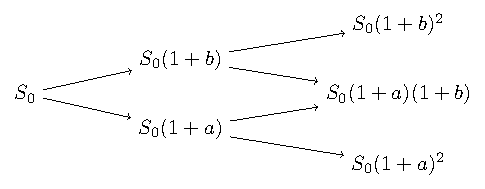
\includegraphics[width=.5\textwidth]{tikz/stochv_1_2_crr.pdf}
	\end{center}
	Man nennt dies auch ein ''rekombinierendes Baummmodell``. Es hat den Vorteil, dass die Anzahl der Knoten nur linear mit $n$ wächst.
	\item Abgezinster Preisprozess $\tilde{S}_n := \frac{S_n}{S_n^0} = S_0 * \prod_{k=1}^n \frac{1+R_k}{1+r}$.
	\item Filtration: natürliche Filtration $\F_n = \sigma \brackets{S_1, \dots, S_n}$.
\end{itemize}

\begin{proposition} %2.1
	Im CRR-Modell gilt:
	\begin{enumerate}
		\item Die Anzahl der Aufwärtsbewegungen $U_n := \# \set{k \in [n] \colon R_k = b}$ ist binomialverteilt, d.h. $U_n \sim \Bin(n,p)$.
		\item Es gilt 
		\begin{align*}
		\log\brackets{\frac{\tilde{S}_n}{S_0}} = U_n \log\brackets{\frac{1+b}{1+a}} + n \log\brackets{\frac{1+a}{1+r}}
		\end{align*}
		d.h. $\log\brackets{\frac{\tilde{S}_n}{S_0}}$ ist nach Skalen-Lagen-Transformation binomialverteilt.
		\item Die Verteilung von $S_n$ ist gegeben durch
		\begin{align*}
		\P\brackets{S_n = S_0 (1+b)^k (1+a)^{n-k}} = \binom{n}{k} p^k (1-p)^{n-k}
		\end{align*} 
	\end{enumerate}
\end{proposition}
\begin{proof}
	\begin{enumerate}
		\item klar
		\item $\frac{\tilde{S}_n}{S_0} = \brackets{\frac{1+b}{1+a}}^{U_n} * \brackets{\frac{1+a}{1+r}}^n \implies \log\brackets{\frac{\tilde{S}_n}{S_0}} = U_n \log\brackets{\frac{1+b}{1+a}} + n \log\brackets{\frac{1+a}{1+r}}$
		\item Es ist $S_n = S_0 (1+b)^{U_1}(1+a)^{n-U_n} $. Also
		\begin{align*}
		\P\brackets{S_n = S_0 (1+b)^k (1+a)^{n-k}} = \P(U_n = k) \overset{(a)}{=} \binom{n}{k} p^k (1-p)^{n-k}
		\end{align*}
	\end{enumerate}
\end{proof}
\begin{*remark}
	Teil (b) suggeriert Konvergenz von $\log\brackets{\frac{\tilde{S}_n}{S_0}}$ gegen Normalverteilung für $n \to \infty$ (nach Skalierung) 
	$\leadsto$ Black-Scholes-Modell ($\nearrow$ Kapitel 3).
\end{*remark}
\begin{lemma} %2.2
	Eine selbstfinanzierende Anlagestrategie $(\eta_n,\xi_n)_{n\in \N}$ mit Anfangskapital $w \in \R$ und Werteprozess $\Pi_n$ sind durch $w$ und $(\xi_n)_{n \in \N}$ vollständig definiert.
	\begin{itemize}
		\item Der diskrete Werteprozess lässt sich darstellen als
		\begin{align*}
		\tilde{\Pi}_n = w + \sum_{k=1}^n \xi_k (\tilde{S}_k - \tilde{S}_{k-1}) = w + (\xi \bigcdot \tilde{S})_n
		\end{align*}
		\item Der Anteil $\eta_n$ ist eindeutig gegeben durch
		\begin{align*}
			\eta_n = \tilde{\Pi}_n - \xi_n \tilde{S}_n
		\end{align*}
	\end{itemize}
\end{lemma}
\begin{proof}
	klar!
\end{proof}
\section{Replikation/Hedging von Derivaten in CRR-Modell}
Derivat $C$ mit Auszahlung $h(S_1, S_2, \dots, S_N)$ zum Zeitpunkt $N$, d.h. $C = h(S_1, S_2, \dots, S_n) \mit h$ messbar.\\
Gesucht ist eine replizierende Strategie $(\xi_n)_{n \in [N]}$ und Anfangskapital $w$, d.h.
\begin{itemize}
	\item $(\xi_n)$ vorhersehbar mit diskreten Werteprozess $\tilde{\Pi}_n = w + (\xi \bigcdot \tilde{S})_n$
	\item Replikationsbedingung
	\begin{align*}
		C = h(S_1, \dots, S_N) = \Pi_N \text{   f.s. } \tag{Rep}\label{eq_2_2_rep}
	\end{align*}
\end{itemize}
\begin{definition}
	\begin{enumerate}
		\item Derivat $C$ heißt \begriff{erreichbar}, wenn eine Replikationsstrategie existiert.
		\item Ein Finanzmodell heißt \begriff{vollständig}, wenn jedes Derivat erreichbar ist.
	\end{enumerate}
\end{definition}
\begin{theorem} %2.3
	Sei $C = h(S_1, \dots, S_N)$ Derivat im CRR-Modell. Dann ist $C$ erreichbar, d.h. $\exists w \in \R$ und $(\xi_n)_{n \in \N}$ mit \eqref{eq_2_2_rep}. Es gilt:
	\begin{enumerate}
		\item $\exists$ messbare Funktion $f_n \colon \R^n \to \R, n \in [N]$ so dass
		\begin{align*}
			\Pi_n = f_n(S_1, \dots, S_n)
		\end{align*}
		und die Werte von $f_n$ entlang der Pfade im Binomialbaums sind rekursiv bestimmt durch
		\begin{align*}
			Rek = \begin{cases*}
				f_N(S_1, \dots, S_N) = h(S_1, \dots, S_N) = C\\
				f_n(S_1, \dots, S_N) = \frac{1}{1+r}\brackets{\frac{r-a}{b-a} f^b_{n+1} + \frac{b-r}{b-a}f^a_{n+1}} \forall n \in [N]_0
			\end{cases*}
		\end{align*}
		wobei $f^b_{n+1} = f_{n+1}(S_1, \dots, S_n(1+b))$ und $f^a_{n+1} = f_{n+1}(S_1, \dots, S_n(1+a))$
		\item Die Replizierende Strategie ist gegeben durch
		\begin{align*}
			\xi_n = \frac{f^b_n - f^a_n}{S_{n-1}(b-a)} \tag{$\Delta$-Hedge}\label{eq_2_3_hedge}
		\end{align*}
	\end{enumerate}
\end{theorem}
\begin{conclusion}
	Das CRR-Modell ist vollständig.
\end{conclusion}
\begin{conclusion}
	Ist $C$ ein europäisches Derivat, d.h. $C = h(S_N)$, mit $h\colon \R \to \R$ messbar, dann gelten folgende Vereinfachungen: Es reicht $f_n \colon \R \to \R$ zu nehmen und es gilt
	\begin{align*}
		\Pi_n = f_n(S_n) \quad f_{n+1}^b = f_{n+1}(S_n(1+b)) \quad f^a_{n+1} = f_{n+1}(S_n(1+a))
	\end{align*}
\end{conclusion}
\begin{*remark}
	\begin{enumerate}
		\item Rekursionen $Rek$ entspricht einem Rückwärtsdurchlauf des Baumdiagramms BILD: *tree diagram is missing :/* $f_n$ wird als diskontierter, gewichteter Mittelwert von $f^b_{n+1}$ und $f^a_{n+1}$ bestimmt. Die Gewichte $q_b = \frac{r-a}{b-a},q_a = \frac{b-r}{b-a}$. Es gilt: $q_a + q_b = 1$
		\item Ursprüngliche Übergangswahrscheinlichkeiten $p$ spielen für Bewertung von $C$ \emph{keine} Rolle: Sie werden durch ``risiko-neutrale'' Wahrscheinlichkeiten $q_b, q_a = 1-q_b$ ersetzt
		\item Lässt sich auf den Computer auch für große Bäume effizient implementieren
		\item Die Formel für $\xi_n$ wir auch als ``Delta-Hedge'' bezeichnet
		\begin{align*}
			\xi_n = \frac{\text{``Preissenkung Derivat''}}{\text{``Preissenkung Basisgut''}} \quad \text{ Differenzenquotient}
		\end{align*}
		\item Weitere Interpretation von $\xi_n$
			\begin{itemize}
				\item $\xi_n > 0$ Preisänderung Derivat hat selbes Vorzeichen wie Preissenkung Basisgut, keine Lehrverkäufe notwendig!
				\item $\xi_n < 0$ Preisänderung Derivat hat entgegengesetztes Vorzeichen wie Preissenkung Basisgut, keine Lehrverkäufe notwendig!
				\item $\xi_n \approx 0$ Preisänderung Derivat hängt kaum von Preisänderung Basisgut ab.
			\end{itemize}
	\end{enumerate}
\end{*remark}
\begin{proof}
	Mittels Rückwärtsinduktion über $n \in [N]_0$ 
	\begin{enumerate}
		\item Für $n \in \N$ gilt: $\Pi_N = C = h(S_1, \dots, S_N)$ \eqref{eq_2_2_rep} also $\Pi_N = f_N(S_1, \dots, S_N)$ mit $f_N = h$
		\item Induktionsschritt aus SF-Bedingung folgt
		\begin{align*}
			&\tilde{\Pi}_{n+1} = \tilde{\Pi}_n = \xi_{n+1}(\tilde{S}_{n+1} - \tilde{S}_n) \quad | (1+r)^{n-1}\\
			&\implies \Pi_{n+1} - (1+r)\Pi_n = \xi_{n+1}(S_{n+1} - (1+r)S_n) \tag{$\ast$}\label{eq_2_4_proof}
		\end{align*}
		Nach IV gilt $\Pi_{n+1} = f_{n+1}(S_1, \dots, S_{n+1}) = f_{n+1}(S_1, \dots, S_n, S_n (1+R_{n+1}))$ (da Definition CRR und $S_{n+1} = S_n(1+R_n)$).  Der zweite Fall $R_k = b$ und $R_k = a$ können jeweils mit strikt postiver Wahrscheinlichkeit eintreten.
		\begin{itemize}
			\item[Fall 1:] $\Pi_{n+1} = F_{n+1}(S_1, \dots, S_n, S_n(1+b)) = f^b_{n+1}$, einsetzen in \eqref{eq_2_4_proof}, gibt
			\begin{align*}
				f^b_{n+1} - (1+r)\Pi_n = \xi_{n+1}S_n(b-r) \tag{I}\label{eq_2_4_I}
			\end{align*}
			\item[Fall 2:] $S_{n+1} = S_n(1-a)$ und $\Pi_{n+1} = f_{n+1}(S_1, \dots, S_n, S_n(1+a)) = f^a_{n+1}$, einsetzen in \eqref{eq_2_4_proof}, gibt
			\begin{align*}
				f^a_{n+1} - (1+r)\Pi_n = \xi_{n+1}S_n(a-r) \tag{II}\label{eq_2_4_II}
			\end{align*}
		\end{itemize}
	$\Pi_n$ ist $\xi_{n+1}$ $\F_n$-messbar, also unabhängig von $R_{n-1} \implies$ \eqref{eq_2_4_II} \eqref{eq_2_4_I}
		\begin{itemize}
			\item \eqref{eq_2_4_II} - \eqref{eq_2_4_I}: $f^b_{n+1} - f^a_{n+1} = \xi_{n+1} S_n(b-a)$, dann $\xi_{n+1} = \frac{f^b_{n+1} - f^a_{n+1}}{S_n(b-a)}$ also \eqref{eq_2_3_hedge} \checkmark
			\item in \eqref{eq_2_4_I} $f^b_{n+1}-(1+r)\Pi_n = \frac{b-r}{b-a}(f^b_{n+1}-f^a_{n+1})$, dann $\Pi_n = \frac{1}{1+r} \brackets{\frac{r-a}{b-r}f^a_{n+1} + \frac{b-r}{b-a}f^a_{n+1}} \implies \eqref{eq_2_2_rep}$ \checkmark
		\end{itemize}
	\end{enumerate}
\end{proof}
\begin{*remark}
	Lineare GLS \eqref{eq_2_4_I} + \eqref{eq_2_4_II} können wir schreiben als
	\begin{align*}
		\begin{pmatrix}
			1+r & b-r \\
			1+r & a-r
		\end{pmatrix} 
		\begin{pmatrix}
			\Pi_n\\
			\xi_{n+1} S_n
		\end{pmatrix} = 
		\begin{pmatrix}
			f^b_{n+1}\\
			f^a_{n+1}
		\end{pmatrix} \tag{LGS-1}\label{eq_LGS_1}
	\end{align*}
\end{*remark}
\begin{*example}
	``Asiatische Call-Option'', Auszahlung:
	\begin{align*}
		C=(\overline{S}_N - K)_+ \mit \overline{S}_N = \frac{1}{1+N}\sum_{k=0}^N S_k
	\end{align*}
	Pfadabhängiges Derivat. Bewertung im CRR-Modell mit $N=2$ mit Parametern:
	\begin{align*}
		b=0,3\quad a=0,3 \quad r = 0,2\quad S_0 = 100\quad K = 100
	\end{align*}
	Binomialbaum:
	\[
		\begin{tikzcd}
			&                          & 169 \\
			& 130 \arrow[ru] \arrow[r] & 91  \\
			100 \arrow[ru] \arrow[r] & 70 \arrow[ru] \arrow[rd] &     \\
			&                          & 49 
		\end{tikzcd}
	\]
	\begin{align*}
		C&=h(S_1,S_2) \mit h = f_2\\
		h(130,169) &= (\frac{399}{3}-100)_+ = 33\\
		h(130,91) &= (\frac{321}{3}-100)_+ = 7\\
		h(70,91) &= (\frac{261}{3}-100)_+ = 0\\
		h(70,49) &= (\frac{219}{3}-100)_+ = 0
	\end{align*}
	Rekursion:\\
	\begin{align*}
		\text{Nebenrechung: }q = \frac{r-a}{b-a} &= \frac{0,4}{0,6} = 2/3 \und 1-a = 1/3\\
		f_1(130) &= \frac{1}{1+r}(q \cdot f^b + (1-q)f^a)\\
		&= \frac{1}{1,1}(2/3 33 + 1/3 7) = \frac{1}{1,1}\cdot 73/3\\
		&\approx 22,12\\
		f_1(70) &= \frac{1}{1,1}(2/3 0 + 1/3 0) = 0\\
		f_0 &= \frac{1}{1,1}(2/3 \frac{1}{1,1} 73/3 + 1/\cdot 0) \approx 13,41
	\end{align*}
	Strategie:
	\begin{align*}
		\xi_2(130) &= \frac{f_2^b - f_2^a}{S_1 (b-a)} = \frac{33-7}{130\cdot 0,6} = \frac{26}{13\cdot 6} = 1/3\\
		\xi_2(70) &= \frac{0-0}{70\cdot 0,6} = 0\\
		\xi_1 &= \frac{f_1^b - f_1^a}{S_0(b-a)} = \frac{\frac{1}{1,1}73/3 - 0}{100\cdot 0,6} = \frac{73}{3\cdot 11 \cdot 6} = \frac{73}{196} \approx 0,37 
	\end{align*}
\end{*example}
\section{Martingale und Arbitrage im CRR-Modell}
Betrachte CRR-Modell auf W-Raum $(\O,\F,\P)$. Setze weiteres W-Maß $\QQ$ auf $(\O,\F)$. D.h. wir lassen die Baumstruktur unverändert, aber ändern die Übergangswahrscheinlichkeit:
\begin{align*}
	\text{ von }p = \P(R_n = b)\\
	\text{ zu }q = \QQ(R_n = b)
\end{align*}
Notation: $\E^{\QQ}[\cdot]$ Erwartungswert unter $\QQ$.
\begin{definition}
	Ein Wahrscheinlichkeitsmaß $\QQ$ auf $(\O,\F)$ heißt äquivalentes Martingalmaß (EMM) für das CRR-Modell, wenn gilt
	\begin{enumerate}
		\item $\QQ\sim \P$ ($\QQ$ äquivalent zu $\P$)
		\item diskreter Preisprozess $(\tilde{S}_n)_{n \in [N]}$ ist $\QQ$-Martingal, d.h.
		\begin{align*}
			\E^{\QQ}[\tilde{S}_{n+1}\mid \F_n] = \tilde{S}_n \quad \forall n \in [N-1]_0
		\end{align*}
	\end{enumerate}
\end{definition}
\begin{erinnerung}
	$\P, \QQ$ Wahrscheinlichkeitsmaße auf $(\O,\F)$
	\begin{itemize}
		\item $\P \sim \QQ :\Leftrightarrow (\P(A) = 0 \Leftrightarrow \QQ(A) = 0 \forall A \in \F$ (Äquivalent)
		\item $\QQ << \P \Leftrightarrow (\P(A) = 0 \implies \QQ(A) = 0 \forall A \in \F$ ($\QQ$ absolut stetig bezüglich $\P$)
		\item Es gilt: $\QQ \sim \P \Leftrightarrow (\QQ << \P \wedge \P << \QQ)$
	\end{itemize}
\end{erinnerung}
\begin{theorem}
	\proplbl{th_2_3}
	\begin{enumerate}
		\item IM CRR-Modell existiert ein EMM genau dann, wenn $a < r < b$ gilt
		\item Das EMM $\QQ$ ist eindeutig und es gilt
		\begin{align*}
			q &:= \QQ(R_n = b) = \frac{r-a}{b-a}\\
			1-q &= \QQ(R_n = a) = \frac{b-r}{b-a} \quad \forall n \in [N]
		\end{align*}
	\end{enumerate}
\end{theorem}
\begin{*remark}
	$q$ und $1-q$ sind genau die risiko-neutralen Gewichte, die in \eqref{eq_2_2_rep} auftauchen
\end{*remark}
\begin{proof}
	Sei $\QQ$ beliebiges Wahrscheinlichkeitsmaß auf $(\O,\F)$. Setze
	\begin{align*}
		q_n &:= \Q(R_n = b\mid \F_{n-1}) \in [0,1]\\
		\E^{\QQ}[\tilde{S}_n \mid \F_{n-1}] &= \E^{\QQ}[\tilde{S}_n \cdot (\frac{1+R_n}{1+r}) \mid \F_{n-1}]\\
		&= \tilde{S}_{n-1}\frac{1}{1+r}\E^{\QQ}[1+R_n \mid \F_{n-1}]\\
		&= \tilde{S}_{n-1} \cdot \frac{1}{1+r}(q_n(1+b) + (1-q_n)(1+a))
		\intertext{Dann}
		(\tilde{S}_{n \in[N]}) \text{ ist $\QQ$-Martingal} \Leftrightarrow\\
		\frac{1}{1+r}(q_n (1+b) + (1-q_n)(1-a) = 1 \quad \forall n\\
		q_n b = (1-q_n)a = r\\
		q_n (b-a) = r-a \implies q_n = \frac{r-a}{b-a}
	\end{align*}
	\begin{align*}
		q_n \in[0,1] \Leftrightarrow a \le r \le b\\
		\QQ \sim \P\colon q_n \in (0,1) \Leftrightarrow a < r < b
	\end{align*}
	d.h. $\QQ$ ist EMM $\Leftrightarrow a < r < b$.
\end{proof}
\begin{theorem}[Risiko-Neutrale Bewertungsformel]
	Sei $C = h(S_1, \dots, S_n)$ Derivat im CRR-Modell mir EMM $\QQ$. Für den Preisprozess $(\Pi_n)_{n \in [N]}$ von $C$ gilt:
	\begin{align*}
		\Pi_n = (1+r)^{-(N-n)}\cdot \E^{\QQ}[C \mid \F_n]
		\intertext{Insbesondere gilt}
		w = \Pi_0 = (1+r)^{-N} \cdot \E^{\QQ}[C]
	\end{align*}
	\emph{In Worten:} Der faire Preis von $C$ ist eindeutig und gegeben durch den diskontieren Erwartungswert von $C$ \emph{unter dem Martingalmaß $\QQ$}.
\end{theorem}
\begin{proof}
	Der Wahrscheinlichkeitsraum für das CRR-Modell ist endlich, d.h. $\abs{\O} = 2^N < \infty$ (also haben endlich viele Pfade im CRR-Modell). Daraus folgt jede Zufallsvariable ist beschränkt und insbesondere $C$ und $(\xi_n)_{n \in [N]}$. Sei $(\xi_n)$ Replikationsstrategie für $C$ mit diskontinuierten Werteprozess $(\tilde{\Pi}_n)$, d.h.
	\begin{align*}
		\tilde{\Pi}_n = w + \sum_{k=1}^n \xi_k (\tilde{S}_k - \tilde{S}_{k-1}) = w+ (\xi \bigcdot \tilde{S})_n
		\intertext{und}
		\tilde{\Pi}_n = (1+r)^{-N}C
	\end{align*}
	$\QQ$ ist EMM $\implies (\tilde{S}_n)$ ist $\QQ$-Martingal. Mit Theorem 1.6 $(\xi \bigcdot \tilde{S})_n$ ist $\QQ$-Martingal. Damit folgt $\tilde{\Pi}_n$ ist $\QQ$-Martingal.
	\begin{align*}
		\Pi_n &= (1+r)^n \cdot \tilde{\Pi}_n = (1+r)^n \E^{\QQ}[\Pi_N \mid \F_n] \quad \text{Martingal}\\
		&= (1+r)^{-(N-n)} \cdot \E^{\QQ}[C \mid \F_n].
	\end{align*}
\end{proof}
\begin{*remark}[zur Martingalbedingung für $\QQ$]
	Wir schreiben (etwas umständlich) 
	\begin{itemize}
		\item $q_b = \QQ(R_n = b)$ und $q_a = \QQ(R_n = a)$
		\item $\QQ$-Maß: $q_a + q_b = 1 \Leftrightarrow q_b(1+r) + q_a (1+r) = 1+r$
		\item Martingalbedingung:
		\begin{align*}
			 (1+b)q_b + (1+a)q_a = 1-r \Leftrightarrow q_b(b-r) + q_a(a-r) = 0
		\end{align*}
		Als LGS:
		\begin{align*}
			\begin{pmatrix}
				1+r & 1+r \\
				b-r & a-r
			\end{pmatrix}
			\begin{pmatrix}
			q_b\\ q_a
			\end{pmatrix} =
			\begin{pmatrix}
				1+r\\ 0
			\end{pmatrix} \tag{LGS-2}\label{eq_2_4_LGS2}
		\end{align*}
		ist Bedingung für Martingalmaß. Vergleiche mit
		\begin{align*}
		\begin{pmatrix}
		1+r & 1+r \\
		b-r & a-r
		\end{pmatrix}
		\begin{pmatrix}
		\Pi_{n+1}\\ \xi_n \cdot S_{n-1}
		\end{pmatrix} =
		\begin{pmatrix}
		f_n^b\\ f_n^a
		\end{pmatrix}
		\end{align*}
		letzteres ist wieder \eqref{eq_LGS_1}, also Gleiche Matrix, aber transponiert $\implies$ \begriff{Dualität}!
	\end{itemize}  
\end{*remark}
\subsection*{Arbitrge im CRR-Model}
\begin{definition}
	Eine Anlagestrategie $(\xi_n)_{n \in[N]}$ mit Zeithorizont $N$ und diskontinuierlichem Werteprozess $(\tilde{\Pi}_n)_{n \in [N]}$ heißt \begriff{Arbitrage}, wenn gilt:
	\begin{enumerate}
		\item $\tilde{\Pi}_0 = 0$ (Kein Anfangskapital)
		\item $\P(\tilde{\Pi}_N \ge 0) = 1$ (kein Verlustrisiko)
		\item $\P(\tilde{\Pi}_N > 0) > 0$ (positiver Gewinn mit positiver Wahrscheinlichkeit)
	\end{enumerate}
	Die 3 Bedingungen nehmen wir (Arb.) % find a way to reference to all 3 :(
\end{definition}
\begin{theorem} %2.8
	\propref{theo_2_8}
	Im CRR-Modell sind äquivalent
	\begin{enumerate}
		\item Es existiert keine Arbitrage (NA = ``No-Arbitrage'')
		\item Ex existiert ein EMM $\QQ$ 
	\end{enumerate}
\end{theorem}
\begin{*remark}
	Dieses Theorem gilt im Wesentlichen in \emph{allen} Finanzmodellen (diskret, stetig, ...). Heißt auch \emph{1. Hauptsatz der Preistheorie}.
\end{*remark}
\begin{proof}
	\begin{itemize}
		\item b)$ \implies$ a) mit Widerspruch. Sei $\QQ$ ein EMM \emph{und} $(\xi)$ Arbitrage. Wegen $\QQ \sim \P$ folgt aus (Arb):
		\begin{align*}
			\QQ(\tilde{\Pi}_N \ge 0) = 1\\
			\QQ(\tilde{\Pi}_N > 0) > 0\\
			\implies \E^{\QQ}[\tilde{\Pi}_N] > 0 \tag{$\ast$}\label{eq_2_4_2_8}
		\end{align*}
		Andererseits: $\tilde{\Pi}_N = 0 + (\xi \bigcdot \tilde{S})_N$. $\tilde{S}$ ist $\QQ$-Martingal $\implies (\xi \bigcdot \tilde{S})$ ist $\QQ$-Martingal, dann
		\begin{align*}
			\E^{\QQ}[\tilde{\Pi}_N] = \E^{\QQ}((\xi \bigcdot \tilde{S})_N) = 0
		\end{align*}
		und das ist ein Widerspruch zu \eqref{eq_2_4_2_8}.
		\item a)$ \implies$ b) klar \checkmark
	\end{itemize}
\end{proof}